\documentclass[12pt]{report}
\usepackage[a4paper,
bindingoffset=0.2in,
left=0.1in,
right=0.1in,
top=0.5in,
bottom=0.5in,
footskip=.25in]{geometry}
\usepackage[utf8]{inputenc}
\usepackage[english,portuguese]{babel}
\usepackage[myheadings]{fullpage}
\usepackage[T1]{fontenc}
\usepackage{fancyhdr}
\usepackage{graphicx, setspace}
\usepackage{sectsty}
\usepackage{url}
\usepackage{pdfpages}
\usepackage{subcaption}
\usepackage{amsmath}
\usepackage{multirow}
\usepackage{tikz}
\usepackage{minted}
\usepackage{hyperref}
\usepackage{amsfonts}
\usepackage{bbm, dsfont}
\usepackage{tikz}
\usepackage{mathtools}
%\usetikzlibrary{positioning}
\usetikzlibrary{shapes,positioning,calc,quotes}
\tikzstyle{subrotina} = [rectangle, draw,text centered, minimum width=5em, inner sep=5pt]
\tikzstyle{funcao} = [rounded rectangle, draw, text centered, minimum width=7em, inner sep=5pt]
\tikzstyle{random} = [rectangle, text centered, inner sep=5pt, minimum width=5em]
\tikzstyle{loop} = [rectangle, draw, align=left]
\tikzstyle{fluxo} = [draw, thick, -latex]
\tikzstyle{meiofluxo} = [draw, -]
\tikzstyle{chamada} = [draw, dashed, <->]


%%------ 
%% Comandos gerais
%% Observação: o arquivo "comandos.tex" tem que estar presente.
%%------
%%%%%%%%%%%%%%%%%%%%%%%%%%%%%%%%%%%%%%%%%%%%%%%%%%%%%%%%%%%%%%%%%%%%%
% In English:
%    This is a list of commands specification for FAPESP reports.
%
% In Portuguese:
%    Esta é uma lista de especificação de comandos para relatórios
% da Fundação de Amparo à pesquisa do Estado de São Paulo (FAPESP).
%
% Author/Autor: André Leon Sampaio Gradvohl, Dr.
% Email:        andre.gradvohl@gmail.com
% Lattes CV:    http://lattes.cnpq.br/9343261628675642
% 
% Last update/Última versão: 11/Sep/2016
%%%%%%%%%%%%%%%%%%%%%%%%%%%%%%%%%%%%%%%%%%%%%%%%%%%%%%%%%%%%%%%%%%%%%%

\def\checkmark{\tikz\fill[scale=0.4](0,.35) -- (.25,0) -- (1,.7) -- (.25,.15) -- cycle;}

\DeclareMathOperator{\diag}{diag}
\DeclareMathOperator{\ai}{Ai}
\DeclareMathOperator{\re}{Re}
\DeclareMathOperator{\im}{Im}
\DeclareMathOperator{\ee}{\rm e}
\DeclareMathOperator{\supp}{supp}
\renewcommand{\Re}{\mathop{\rm Re}}
\newcommand{\res}{\mathop{\rm Res}}
\renewcommand{\Im}{\mathop{\rm Im}}
\newcommand{\N}{\mathbb{N}}
\newcommand{\C}{\mathbb{C}}
\DeclareMathOperator{\Tr}{Tr}
\newcommand{\R}{\mathbb{R}}
\newcommand{\Z}{\mathbb{Z}}
\newcommand{\D}{\mathbb{D}}
\newcommand{\Q}{\mathbb{Q}}
\newcommand{\boh}{\mathit{o}}
\newcommand{\Boh}{\mathcal{O}}
\newcommand{\bbp}{\bm K_{\mathrm{BBP}}}
\newcommand{\ii}{\mathrm{i}}
\newcommand{\dd}{\mathrm{d}}
\newcommand*{\deff}{\mathrel{\vcenter{\baselineskip0.5ex \lineskiplimit0pt
			\hbox{\scriptsize.}\hbox{\scriptsize.}}}%
	=}
\newcommand*{\revdeff}{=\mathrel{\vcenter{\baselineskip0.5ex \lineskiplimit0pt
			\hbox{\scriptsize.}\hbox{\scriptsize.}}}%
}

\newcommand{\HRule}[1]{\rule{\linewidth}{#1}}
\setcounter{tocdepth}{3}
\setcounter{secnumdepth}{3}

\newcommand{\titulo}[1]{\def\meuTitulo{#1}}
\newcommand{\tituloIngles}[1]{\def\meuTituloIngles{#1}}
\newcommand{\numProjeto}[1]{\def\numFAP{#1}}
\newcommand{\tipoRelatorio}[1]{\def\tipoRelat{#1 }} %o espaço depois do #1 é importante
\newcommand{\modalidadeProjeto}[1]{\def\modProjeto{#1}} 
\newcommand{\agFomento}[2]{\def\agFom{#1} \def\siglaAgFom{#2}} %extenso Sigla
\newcommand{\autor}[1]{\def\nomeAutor{#1}}
\newcommand{\cidade}[1]{\def\nomeCidade{#1}}
\newcommand{\universidade}[1]{\def\nomeUniversidade{#1}}
\newcommand{\faculdade}[1]{\def\nomeFaculdade{#1}}
\newcommand{\periodoVigencia}[1]{\def\periodVig{#1}}
\newcommand{\periodoRelatorio}[1]{\def\periodRelat{#1}}

\author{}
\date{}

%Definição de membros da equipe de pesquisas
\newcommand{\membroA}[1]{\def\nomeMembroA{#1}}
\newcommand{\membroB}[1]{\def\nomeMembroB{#1}}
\newcommand{\membroC}[1]{\def\nomeMembroC{#1}}
\newcommand{\membroD}[1]{\def\nomeMembroD{#1}}
\newcommand{\membroE}[1]{\def\nomeMembroE{#1}}
\newcommand{\membroF}[1]{\def\nomeMembroF{#1}}

\newcommand{\Figure}[1]{Figura~\ref{fig:#1}}
\newcommand{\Table}[1] {Tabela~\ref{#1}}
\newcommand{\Equation}[1] {Equa\c{c}\~ao~\ref{#1}}
\newcommand{\addFigure}[3] { %Parametros scale, fig_name, caption 
    \begin{figure}[!hbt]
      \centering
      \includegraphics[scale=#1]{figures/}
      \caption{#3}\label{fig:#2}
    \end{figure}
}

\newcommand{\geraTitulo}{
\clearpage
\begin{titlepage}
  \begin{center}
      \vspace*{-3cm}
       { \setstretch{.5} 
         \textsc{\nomeUniversidade} \\
         \HRule{.2pt}\\
         \textsc{\nomeFaculdade}
       }

       \vspace{5.5cm}

       \Large \textbf{\textsc{\meuTitulo}}
 	  \HRule{1.5pt} \\ [0.5cm]
       \linespread{1}
       \large Relatório Científico 
       \ifdefined\tipoRelat
            \tipoRelat
       \fi
       do projeto 
       \ifdefined\modProjeto
           na modalidade \modProjeto,
       \fi
       fomentado pela \agFom. \\ 
   	   \HRule{1.5pt} \\ [0.5cm]

       \ifdefined\numFAP
          Projeto \siglaAgFom~\texttt{\#\numFAP}
          \\ [0.5cm]
       \fi
        Pesquisador Responsável: \nomeAutor
        
        \hspace{2cm}
        
        
\includegraphics[scale=0.7]{Assets/CuteCircleWhite}
       
        \vfill
       
        {\normalsize  \nomeCidade, \today}
 \end{center}
 \end{titlepage}
}

\usepackage{titlesec}
\titleformat{\chapter}{\normalfont\LARGE\bfseries}{\thechapter}{1em}{}
\titlespacing*{\chapter}{0pt}{3.5ex plus 1ex minus .2ex}{2.3ex plus .2ex}

%----------------------------------------------------------------------
% Cabeçalho e rodapé
%----------------------------------------------------------------------
\pagestyle{fancy}
\fancyhf{} % Limpa todos os campos de header and footer fields
\renewcommand{\headrulewidth}{0pt}
\fancyfoot[R]{\thepage}

\addto\captionsportuguese{\renewcommand{\contentsname}{Sumário}}
\addto\captionsportuguese{\renewcommand{\bibname}{Referências Bibliográficas}}

%------
% Resumo e Abstract
%------
\newcommand{\Resumo}[1]{
   \begin{otherlanguage}{portuguese}
       \addcontentsline{toc}{chapter}{Resumo}
       \begin{abstract} \thispagestyle{plain} \setcounter{page}{2}
          #1
        \end{abstract}
   \end{otherlanguage} 
} %end \Resumo

\newcommand{\Abstract}[1]{
   \begin{otherlanguage}{english}
      \addcontentsline{toc}{chapter}{Abstract}
      \begin{abstract} \thispagestyle{plain} \setcounter{page}{3}
       #1
      \end{abstract}    
    \end{otherlanguage} 
} %end \abstract

%------
% Folha de rosto
%------
\newcommand{\folhaDeRosto}{
   \chapter*{Informações Gerais do Projeto}
   \addcontentsline{toc}{chapter}{Informações Gerais do Projeto}
   \begin{itemize}
      \item Título do projeto: 
            \begin{itemize}\item[] \textbf{\meuTitulo} \end{itemize}
      \item Nome do pesquisador responsável: 
            \begin{itemize}\item[]\textbf{\nomeAutor}\end{itemize}
      \item Instituição sede do projeto: 
            \begin{itemize}
               \item[]\textbf{\nomeFaculdade \ da \nomeUniversidade} 
            \end{itemize}
      \item Equipe de pesquisa:
            \begin{itemize}
               \ifdefined\nomeMembroA
                 \item[]\textbf{\nomeMembroA}
               \else 
                 \item[]\textbf{\nomeAutor}
               \fi
               \ifx\nomeMembroB\undefined\else \item[]\textbf{\nomeMembroB}\fi
               \ifx\nomeMembroC\undefined\else \item[]\textbf{\nomeMembroC}\fi
               \ifx\nomeMembroD\undefined\else \item[]\textbf{\nomeMembroD}\fi
               \ifx\nomeMembroE\undefined\else \item[]\textbf{\nomeMembroE}\fi
               \ifx\nomeMembroF\undefined\else \item[]\textbf{\nomeMembroF}\fi
             \end{itemize}
       
          \ifdefined \numFAP
             \item Número do projeto de pesquisa:
             \begin{itemize}
                 \item[]\textbf{\numFAP} 
             \end{itemize}
          \fi  
       \item Período de vigência:
            \begin{itemize}
               \item[]\textbf{\periodRelat} 
            \end{itemize}
       \item Período coberto por este relatório científico:
            \begin{itemize}
               \item[]\textbf{\periodVig} 
            \end{itemize}
   \end{itemize}
   \clearpage
}


\newcommand\underrel[2]{\mathrel{\mathop{#2}\limits_{#1}}}

\newcommand{\matriz}[1]{\hat#1}

\newcommand{\many}[2]{$#1_1, #1_2, \dots, #1_#2$}

\newcommand{\cmany}[3]{$#1_1 #3 #1_2 #3 \dots #3 #1_#2$}

\newcommand{\mmany}[2]{ #1_1, #1_2, \dots, #1_#2 }

\newcommand{\mcmany}[3]{#1_1 #3 #1_2 #3 \dots #3 #1_#2}

\newcommand{\set}[1]{\{#1\}}

\newcommand{\cjgt}[1]{\overline{#1}}
\DeclareMathOperator{\sign}{sign}
\DeclareMathOperator{\Df}{D}
\DeclareMathOperator{\Ee}{E}
\DeclareMathOperator{\h}{h_1}
\DeclareMathOperator{\f}{f}
\DeclareMathOperator{\U}{U}
\DeclareMathOperator{\W}{W}
\DeclareMathOperator{\K}{K}
\DeclareMathOperator{\Hf}{\mathcal{H}}
\DeclareMathOperator{\Qf}{Q}
\DeclareMathOperator{\Gl}{\mathcal{L}}
\DeclareMathOperator{\g}{g}
\DeclareMathOperator{\V}{V}
\newcommand{\iu}{\mathrm{i}\mkern1mu}
\renewcommand{\Im}{\mathop{\textrm Im}}
\newcommand{\J}{J} %Jacobiano
\newcommand{\Id}{\mathbb{1}}
\newcommand{\p}{\mathcal{P}} %medida
\newcommand{\Se}{\mathbb{S}}
\newcommand{\He}{\mathbb{H}}
 \newcommand{\E}{\mathbb{E}}

% MATH DECLARATIONS
\newtheorem{lemma}{Lema}[section]
\newtheorem{thm}[lemma]{Teorema}
\newtheorem{claim}[lemma]{Afirmação}
\newtheorem{cor}[lemma]{Corolário}
\newtheorem{definition}[lemma]{Definição}
\newtheorem{conjecture}[lemma]{Conjectura}
\newtheorem{prop}[lemma]{Proposição}
\newtheorem{assumption}[lemma]{Assumpção}
\numberwithin{equation}{section} %numeracao dentro de secoes

% PROOF ENV
\makeatletter
\newenvironment{proof}[1][Demonstração]{\par
	\pushQED{\qed}%
	\normalfont \topsep6\p@\@plus6\p@\relax
	\trivlist
	\item\relax
	{\itshape
		#1\@addpunct{.}}\hspace\labelsep\ignorespaces
}{%
	\popQED\endtrivlist\@endpefalse
}
\makeatother
%%-----
%% Página de título
%% Observação: As definições que aparecem a seguir comporão a
%%             página de título e a folha de rosto.
%%-----
%% Define o nome da universidade onde o projeto foi desenvolvido.
\universidade{Universidade de São Paulo}
%
%% Define o nome da faculdade onde o projeto foi desenvolvido.
\faculdade{Instituto de Ciências Matemáticas e de Computação (ICMC)}
%
%% Define o título do projeto.
\titulo{Matrizes aleatórias e simulação de gases de Coulomb}
%
%% Define a agencia de Fomento e a abreviatura. O primeiro argumento é o 
%% nome por extenso e o segundo a abreviatura.
%% Ambos os argumentos são obrigatórios
\agFomento{Fundação de Amparo à Pesquisa do Estado de São Paulo}{FAPESP}
%
%% Define o tipo de relatório. Pode ser Anual ou Final.
%% Não é obrigatório definir o tipo de relatório.
\tipoRelatorio{Final}
%
%% Define a modalidade de Projeto. Pode ser temático, regular, etc.
\modalidadeProjeto{Iniciação Científica}
%
%% Define o número do projeto.
%% Não é obrigatório definir o número do projeto.
\numProjeto{2023/02674-0} 
%
%% Define o autor do relatório.
\autor{Guilherme L. F. Silva}
%
%% Define a equipe do projeto (incluindo o pesquisador responsável no comando \membroA{}
\membroA{Guilherme L. F. Silva}
%% Inclua os demais membros do grupo (máximo +5)
\membroB{João Victor Alcantara Pimenta}
%\membroC{Francisco}
%\membroD{Joao}
%\membroE{Antonio}
%\membroF{José}
%
%% Define o período da vigência do Projeto.
\periodoRelatorio{01/06/2023 a 31/05/2024}
%
%% Define o período coberto pelo relatório.
\periodoVigencia{01/06/2023 a 31/05/2024}
%
%% Define a cidade onde o projeto foi desenvolvido.
\cidade{São Carlos}

%%-----
%% Página de título
%% Observação: Os comandos a seguir não devem ser mudados, 
%%             exceto caso necessário.
%%-----
\begin{document}
%
%% Define a numeração em romanos.
\pagenumbering{roman}
%
%% Gera a folha de título.
\geraTitulo
%
%% Gera a folha de rosto.
\folhaDeRosto
%
%% Escreva aqui o resumo em português.
\Resumo{
  O estudo de Matrizes Aleatórias demonstra aplicabilidade em uma gama diversa de áreas, com
  destaque no estudo de mecânica estatística, principalmente na simulação de gases. Estudando a
  densidade espectral de sistemas de matrizes Gaussianas pode-se desenvolver uma analogia que
  possibilita a simulação de sistemas de gases diversos, como o de Coulomb. Algumas dificuldades
  surgem na implementação de simulações baseadas nesta teoria, principalmente em escalabilidade do sistema e no tratamento de possíveis singularidades. Para resolver estes problemas,
  abordou-se na simulação na literatura, dentre outros, o Algoritmo Híbrido de Monte Carlo, de
  ótimo comportamento numérico. Nosso objetivo é explorar este assunto, as simulações de gases
  e o algoritmo citado acima além de expandir os potenciais em que foi-se bem documentado o
  comportamento destas simulações.
  }
%
%% Escreva aqui o resumo em inglês.
% \Abstract{
%	The study of Random Matrices demonstrates applicability in a diverse range of areas, empha-
%	sizing the study of statistical mechanics, mainly in the simulation of gases. By studying the
%	spectral density of Gaussian matrix systems, one can develop the simulation of Coulomb gas
%	systems in analogy. Some difficulties arise in implementing simulations based on this theory,
%	mainly in system scalability and the treatment of possible singularities. To solve these pro-
%	blems, the literature has simulated these gases, with excellent numerical behavior, using the
%	Monte Carlo Hybrid Algorithm. We wish to explore this problem, the simulations, and the
%	proposed algorithm along with extending the potentials to wich it has been tested.
%}
%
%% Adicionará o sumário.
%% Mantenha o \thispagestyle{empty} e \clearpage
\thispagestyle{empty}
\clearpage
%
%% Define a numeração em arábicos.
\pagenumbering{arabic}

%%-----
%% Formatação do título da seção
%%-----
\sectionfont{\scshape}

%%-----
%% Corpo do texto
%%-----

\chapter{Atividades Desenvolvidas}
\label{section:atividadesdesenvolvidas}

A execução do projeto foi dividida nas seguintes etapas:

\begin{enumerate}
	\item \textbf{Revisão da Literatura em RMT, e estudo de teoria básica do GUE}, é necessário fazer vasta revisão de literatura no tema para que o aluno tenha domínio das ferramentas e métodos utilizados para o tratamento de matrizes aleatórias e suas implicações em mecânica estatística. Para isso, durante esse período será realizado o estudo da bibliografia adequada;
	
	\item \textbf{Estudo dos métodos de Simulação}, como mencionado, uma das aplicações importantes da teoria de matrizes aleatórias reside em sua conexão com gases de Coulomb. Em 2018 publicou-se o artigo \cite{Chafa2018}, base para o estudo do método de simulação implementado;
	
	\item \textbf{Implementação dos algoritmos}, implementa-se os métodos descritos no artigo e tenta-se estender seu uso em condições diferentes das utilizadas no artigo, como por exemplo em outros potenciais;
	
	\item \textbf{Redação dos Relatórios Científicos}, quando serão escritos os relatórios exigidos pelas normas da \textit{FAPESP}.
	
\end{enumerate}

\section{Cronograma}

Com base nas tarefas enumeradas na Seção \ref{section:atividadesdesenvolvidas}, é mostrado na Tabela \ref{tab:cronograma1ano} o cronograma atual de desenvolvimento do projeto. Foi possível realizar todo o planejamento feito inicialmente.

%\begin{table}[ht]
%\centering
%\begin{tabular}{|c|c|c|c|c|c|c|c|c|c|c|c|c|}
%\hline
%\multirow{2}{*}{{\bf Fases}} & \multicolumn{6}{c|}{{\bf Meses}}
%\\ \cline{2-7}
%    & 1 & 2 & 3 & 4 & 5 & 6
%\\ \hline
%    {\bf 1. Revisão Literatura RMT} & x & x & x & & &  
%\\ \hline
%    {\bf 2. Métodos de Simulação} &  &  & x & x & &
%\\ \hline
%    {\bf 3. Implementação algoritmos} & & & & x & x & 
%\\ \hline
%    {\bf 4. Redação Relatórios} & & & & & & x
%\\ \hline
%\end{tabular}
%\caption{Cronograma das atividades.}
%\label{tab:cronograma6meses}
%\end{table}

\begin{table}[ht]
	\centering
	\begin{tabular}{|c|c|c|c|c|c|c|c|c|c|c|c|c|}
		\hline
		\multirow{2}{*}{{\bf Fases}} & \multicolumn{12}{c|}{{\bf Meses}}
		\\ \cline{2-13}
		& 1 & 2 & 3 & 4 & 5 & 6 & 7 & 8 & 9 & 10 & 11 & 12
		\\ \hline
		{\bf 1. Revisão Literatura RMT} & \checkmark & \checkmark & \checkmark & \checkmark & \checkmark & & & & & & &
		\\ \hline
		{\bf 2. Métodos de Simulação} &  &  &  & \checkmark & \checkmark & \checkmark & \checkmark & \checkmark & & & &
		\\ \hline
		{\bf 3. Implementação algoritmos} & & & & & \checkmark & \checkmark & \checkmark & \checkmark & \checkmark & \checkmark & \checkmark &
		\\ \hline
		{\bf 4. Redação Relatórios} & & & & \checkmark & \checkmark & & & & & & \checkmark & \checkmark 
		\\ \hline
	\end{tabular}
	\caption{Cronograma das atividades.}
	\label{tab:cronograma1ano}
\end{table}

\chapter{Realizações do período}\label{chp:realizacoes}

\section{Graduação}

Durante o período referente à pesquisa o aluno realizou as seguintes matérias e respectivos desempenhos:
\hspace{1cm}

\begin{center}
	\begin{tabular}{|c|c|c|c|}
		\hline
		Disciplina & Sigla & Nota & Semestre \\
		\hline
		Mecânica Estatística Avançada & 7600041 & 10.0 & 1 - 2023 \\
		\hline
		Introdução aos Sistemas de Computação & 7600056 & 9.2 & 1 - 2023 \\
		\hline
		Física Estatística Computacional & 7600073 & 9.7 & 1 - 2023 \\
		\hline
		Teoria Espectral de Matrizes & SME0243 & 10.0 & 1 - 2023 \\
		\hline
		Mecânica Quântica & 7600022 & 9.3 & 2 - 2023 \\
		\hline
		Física Matemática Avançada & 7600034 & 10.0 & 2 - 2023 \\
		\hline
		Noções Básicas de Fabricação Mecânica & 7600134 & 10.0 & 2 - 2023 \\
		\hline
		Espaços Métricos & SMA0343 & 9.0 & 2 - 2023 \\
		\hline
		Laboratório Avançado de Física 1& 7600024 & - & 1 - 2024 \\
		\hline
		Álgebra 1 & SMA0305 & - & 1 - 2024 \\
		\hline
		Trabalho de Conclusão de Curso & 7600039 & - & 1 - 2024 \\
		\hline
	\end{tabular}
\end{center}

\section{Participação em eventos científicos}\label{chp:particEvento}

Durante o período de 13 de Janeiro à 24 de Fevereiro o bolsista participou do evento ``Jornadas de Pesquisa em Matemática'' realizado pelo Instituto de Ciências Matemáticas e de Computação (ICMC - USP). Durante este evento foi realizado pesquisa original em simulações de caminhos aleatórios, que rendeu o relatório de nome 'Baralhos e passeios aleatórios', submetido para a FAPESP e disponível em anexo.

O bolsista também apresentou em dois eventos no período da pesquisa. O Colóquio Brasileiro de Matemática (CBM) e a Semana Integrada da Física de São Carlos (SIFSC). Apenas para o primeiro, realizado no Rio de Janeiro, foi necessário o uso da reserva técnica. Por isso, segue o pôster apresentado na próxima página. O trabalho é complementar aos estudos assintóticos e de probabilidade realizados nos meses cobertos por este relatório.

\hspace{1cm}

\begin{center}
\begin{tabular}{|c|c|c|c|c|c|}
	\hline
	Evento &  Sede & Data & Modalidade & Apresentação & Reserva Técnica \\
	\hline
	CBM & IMPA & 24-28/07/23 & Presencial & Pôster - Oral & Sim \\
	\hline
	SIFSC & IFSC-USP & 21-25/08/23 & Presencial & Pôster - Oral & Não \\
	\hline
	Jornadas & ICMC-USP & 13/01-24/02/23 & Presencial & Oral & Não \\
	\hline
\end{tabular}
\end{center}

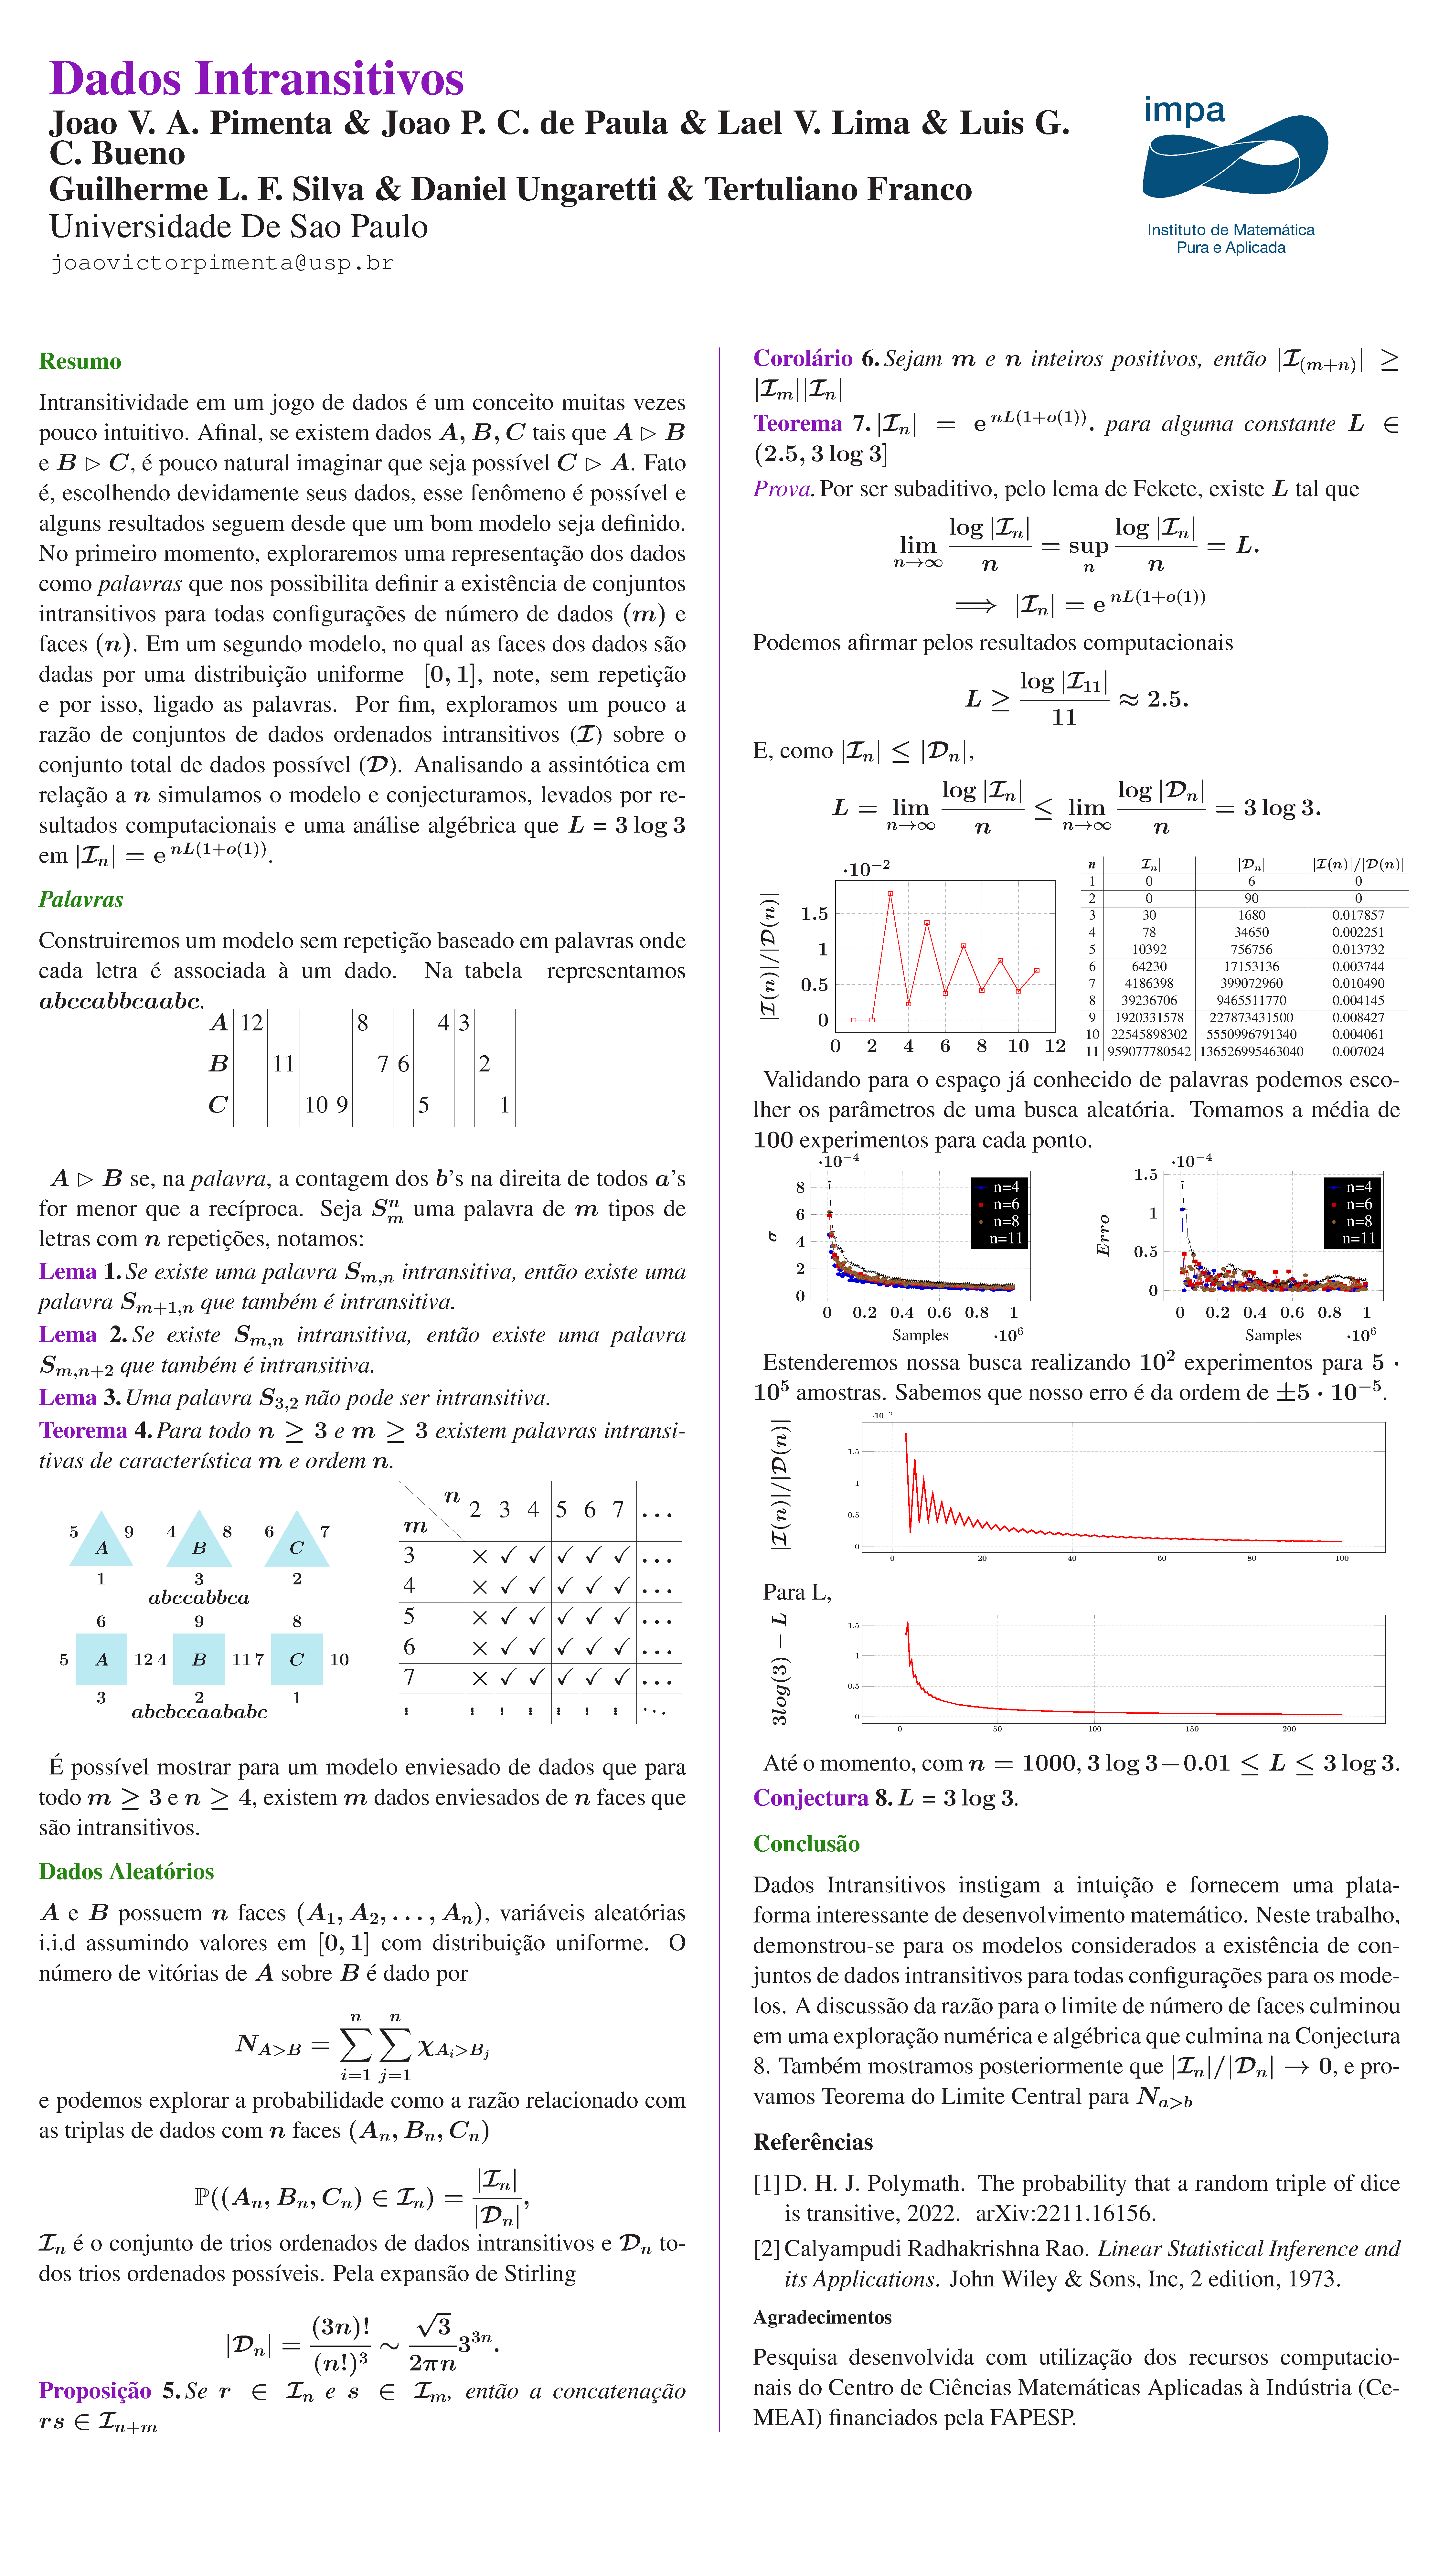
\includepdf[pages={1}]{Assets/posterwhite.pdf}

\section{Outros trabalhos Preparados ou Submetidos}

Durante o período da bolsa foi também finalizado o trabalho intitulado ``A Central Limit Theorem for intransitive dice'' co-autorado pelo aluno beneficiário da bolsa. O arquivo se encontra disponível
na plataforma Arxiv em \url{https://arxiv.org/abs/2310.17083} e está em processo de publicação. Por fim, realizou-se também o desenvolvimento do Trabalho de Conclusão de Curso referente à graduação em andamento. A ser defendido, disponível em anexo.

\section{Pesquisa}
\label{Pesquisa}

Os resultados e texto científico abaixo foram desenvolvidos conjuntamente com o trabalho de conclusão de curso realizado no mesmo período, tomando como base seu conteúdo. Apresento breve noção do tema de trabalho e alguns resultados e possibilidades para desenvolvimento e uso destes. Todos os produtos, programas e textos, podem ser acessados em \url{https://github.com/Joao-vap/RMT-TEX} e \url{https://github.com/Joao-vap/RMT-Code}.

\subsection{Matrizes Aleatórias}
\label{Section: Matrizes}

Sistemas integráveis em física são descritos por equações diferenciais simples o suficiente tais que se pode determinar soluções explícitas. Seu comportamento é, em algum sentido, previsível e unicamente determinado pelas condições iniciais. Naturalmente, muitos sistemas de interesse não se enquadram nessa classe, são chamados caóticos ou não integráveis. Seja por complexidade ou instabilidade, não conseguimos expressar ou resolver significativamente os operadores associados a esses sistemas. 

De acordo com a mecânica quântica, níveis de energia de um sistema são descritos pelos autovalores de seu operador hermitiano associado, o Hamiltoniano $\Hf$. Para um modelo simples o suficiente, caracterizar o sistema físico é equivalente a resolver o problema de autoenergias $\Hf \Psi_i = E_i \Psi_i$. Contudo, para estados excitados de alta energia de núcleos atômicos pesados, por exemplo, esta abordagem se torna impeditiva: ou não se sabe o Hamiltoniano, ou sua solução é complicada. Wigner sugere uma abordagem alternativa, estatística, para o problema de autovalores. Tal teoria descreveria as propriedades estatísticas da estrutura energética nucleica ao invés de detalhar seus níveis. Buscava-se, em algum sentido, uma universalidade, uma descrição que fosse, dada complexidade o suficiente, sensível às simetrias, mas independente dos detalhes em $\Hf$. A teoria foi prontamente seguida por, dentre outros, Gaudin, Mehta, \cite{MehtaGaudin} e Dyson, \cite{Dyson} que avançaram na descrição dos principais ensembles. Esse desenvolvimento é o início do que chamamos hoje Teoria de Matrizes Aleatórias (RMT, \textit{Random Matrix Theory}).

Seja $\Se$ um conjunto tal como $\R, \C, \He $ (Reais, Complexos e Quaterniônicos). Consideremos inicialmente uma matriz $\matriz{M} \in \mathcal{M}_{\Se}(N)$ espaço de matrizes $N \times N$, de entradas reais, complexas ou quaterniônicas. Se tomamos o elemento de matriz $M_{i,j}$ $\forall i, j \in \Z$, com $1 \leq i, j \leq N$, como variável aleatória de distribuição arbitrária, podemos expressar a densidade de probabilidade conjunta de $\matriz{M}$ (jpdf, \textit{joint probability density function}) como $$\p(\hat{M}) \dd \matriz{M} = \p(M_{1,1}, \dots, M_{N,N}) \prod_{i,j=1}^{N} \dd M_{i,j}.$$

Considere a decomposição nas coordenadas espectrais $\matriz{M} = \matriz{P} \matriz{\Lambda} \matriz{P}^{-1}$ onde $\matriz{P}$ é matriz invertível e $\matriz{\Lambda} = \diag(\mmany{\lambda}{N})$. Para que valha a decomposição tomaremos $\matriz{M}$ matriz simétrica, hermitiana ou hermitiana quaterniônica. Esta escolha é feita em importantes ensembles em RMT e motivada fisicamente sabendo que, para sistemas quânticos invariantes reversíveis, o Hamiltoniano é matriz real simétrica; na presença de campo magnético, o Hamiltoniano é matriz complexa hermitiana; na presença de acoplamento spin-órbita, o Hamiltoniano é matriz hermitiana quaterniônica. \cite[Capítulo~2]{RMT-firstcourse-Potters} Devemos atentar ainda pela escolha de mapa $\matriz{M} \mapsto \matriz{P} \matriz{\Lambda} \matriz{P^{-1}}$ bijetivo\footnote{Injetividade é garantida desconsiderando fase e sinal dos autovetores e ordenando os autovalores. Restringe-se ao subconjunto de matrizes sem multiplicidade de autovalores - denso, aberto e de medida completa tal que seu complemento é irrelevante na integração conseguinte.}. Se a mudança de variáveis tem Jacobiano $\J(\matriz{M} \rightarrow \{ \matriz{\Lambda}, \matriz{P} \} )$, reescreve-se a jpdf em função de $\matriz{\Lambda}$ e $\matriz{P}$ tal que
\begin{equation}
	\p(\hat{M}) \dd \matriz{M} = \p \left( M_{1,1}(\matriz{\Lambda}, \matriz{P}), \cdots, M_{N,N}(\matriz{\Lambda}, \matriz{P}) | \J(\matriz{M} \rightarrow \{ \matriz{\Lambda}, \matriz{P} \} ) \right) \dd \matriz{\Lambda} \dd \matriz{P}.
	\label{Equation: p(lambda, O)}
\end{equation}

Estamos especialmente interessados na distribuição de autovalores, logo, devemos integrar a Equação \eqref{Equation: p(lambda, O)} sobre $\dd \matriz{P}$, o que nem sempre é fácil ou possível. Por isso, tomaremos ensembles denominados invariantes (por rotação), isto é, tais que quaisquer duas matrizes $\matriz{M}$ e $\matriz{M'}$ que satisfaçam a relação de equivalência $\matriz{M} = \matriz{U} \matriz{M'} \matriz{U}^{-1}$, sendo $\matriz{U}$ uma rotação, tem mesma probabilidade. Com isso, a jpdf de suas entradas pode ser escrita exclusivamente como função dos autovalores, ou seja, $$\p(\matriz{\Lambda}, \matriz{P}) \dd \matriz{\Lambda} \dd \matriz{P} \coloneqq \p \left( M_{1,1}( \matriz{\Lambda}), \cdots, M_{N,N}(\matriz{\Lambda}) | \J(\matriz{M} \rightarrow \{\matriz{\Lambda}\} ) \right) \dd \matriz{\Lambda} \dd \matriz{P}.$$

Pelo Lema de Weyl, uma jpdf invariante pode ser expressa totalmente por $\p(\matriz{M}) \coloneqq \phi \left(\Tr(V(\matriz{M})) \right)$ com $V$ função polinomial. Além disso, o jacobiano $\J(\matriz{M} \rightarrow \{\matriz{\Lambda}, \matriz{P}\} )$ desta transformação pode ser expresso pelo determinante de matriz de Vandermonde tal que $$\p(\matriz{\Lambda}, \matriz{P}) \dd \matriz{\Lambda} \dd \matriz{P} = \phi \left(\Tr(V(\matriz{M})) \right) \prod_{i<j}^{N} |\lambda_i - \lambda_j|^{\beta} \dd \matriz{\Lambda} \dd \matriz{P},$$ onde $\beta = 1,2,4$ quando tomado $\Se = \R, \C, \He$, respectivamente. Com esta expressão, sabendo medida uniforme sobre os autovetores, podemos explicitar pela primeira vez a jpdf para os autovalores ordenados destes ensembles de matrizes aleatórias como 
\begin{equation}
	\p_{ord}(\mmany{\lambda}{N}) = \frac{1}{Z_{N, \beta}^{(ord)}} \phi{\left( \sum_i^N V(\lambda_i) \right)} \prod_{i < j}^{N} |\lambda_i - \lambda_j|^{\beta}.
	\label{Equation: p-ord}
\end{equation}

Note que, graças ao jacobiano, autovalores destas matrizes apresentam repulsão mútua, expressa pelo produtório na Equação \eqref{Equation: p-ord}. Este fato naturaliza a analogia da Seção \ref{Section: Gases de Coulomb} e é central a muitos resultados em RMT. É possível fazer desenvolvimento análogo para matrizes normais de ensembles associados a $\beta = 2$ com autovalores $\lambda_i \in \C$ - extensão explorada nos resultados. Outros casos fogem ao escopo do trabalho.

Dentre os muitos ensembles em RMT, os Gaussianos são notórios. São eles o \textit{Gaussian Orthogonal Ensemble (GOE)} ($\beta=1$), \textit{Gaussian Unitary Ensemble (GUE)} ($\beta=2$) e \textit{Gaussian Sympletic Ensemble (GSE)} ($\beta=4$). Notemos primeiramente que o nome é relacionado à escolha de $\Se$. Mais explicitamente, o nome é dado em relação à se $\matriz{O}$, tal que $\matriz{M} = \matriz{O}\matriz{\Lambda}\matriz{O}^{-1}$, é ortogonal, unitário ou simplético. É natural então pensar nos ensembles \textit{GOE}, \textit{GUE} e \textit{GSE} como matrizes $\matriz{M} \in \mathcal{M}_{\Se}(N)$ onde 
$$
\mathcal{M}_{\Se}(N) \ni M_{i,j} \sim
\begin{cases}
	\mathcal{N}_{\Se}(0,1/2) &  \ \text{para} \ i \neq j,\\
	\mathcal{N}_{\Se}(0,1) & \ \text{para} \ i = j.
\end{cases}
$$

Os três ensembles gaussianos compartilham de uma propriedade exclusiva - são os únicos ensembles com entradas independentes e, simultaneamente, jpdf rotacionalmente invariante. Podemos deduzir, para $\beta = 1,2,4$ que
\begin{equation}
	\p(\vec{\lambda}) = \frac{1}{Z_{N, \beta}} \ee^{-\beta_N \mathcal{H}_N(\vec{\lambda})},
	\label{Equation: medida Gaussian}
\end{equation}
onde $Z_{N, \beta}$ é função de partição canônica para autovalores desordenados\footnote{Usa-se do fator de contagem de Boltzmann para escrever $ Z_{N, \beta} = N! Z_{N, \beta}^{(ord)}$.}, normalizante da Expressão \eqref{Equation: medida Gaussian}. O fator $\beta_N = \beta N^2$ é pensado como a temperatura inversa. Definimos ainda o Hamiltoniano $$\mathcal{H}_N(\vec{\lambda}) = \frac{1}{N}\sum_{i = 1}^{N} \frac{\lambda_i^2}{2} + \frac{1}{N^2} \sum_{i < j} \log{\frac{1}{|\lambda_i - \lambda_j|}}$$ com  $\lambda_i \mapsto \lambda_i \sqrt{\beta N}$.

\subsection{Gases de Coulomb}
\label{Section: Gases de Coulomb}

Para os ensembles que chamamos invariantes, a densidade de autovalores guarda uma importante analogia, a de Gases de Coulomb. Pensando os $N$ autovalores das matrizes como partículas de um gás com o devido núcleo de interação e potencial externo, podemos usar de noções físicas para intuir seu comportamento. Usando das estabelecidas leis termodinâmicas é possível ainda derivar, por exemplo, as densidades de autovalores no limite termodinâmico ($N \rightarrow \infty$). Generalizando o potencial aplicado podemos ainda recuperar um ensemble de matrizes que pode não estar diretamente disponível.

% Sabemos então, que a partir dessa função podemos retirar importantes propriedades estatísticas (macroscópicas) do sistema de autovalores dos ensembles Gaussianos.

O gás de coulomb $\p_N$ é a medida de probabilidade de Boltzmann-Gibbs dada em $(\R^d)^N$ por 
\begin{equation}
	\dd \p_N(\vec{x}) = \frac{e^{-\beta N^2 \Hf_N(\vec{x})}}{Z_{N,\beta}} \dd \vec{x},
	\label{Equação: Medida Gas de Coulomb}
\end{equation}
onde $$\Hf_N(\vec{x}) = \frac{1}{N} \sum_{i = 1}^{N} \V(x) + \frac{1}{2N^2} \sum_{i \neq j} \g(x_i - x_j)$$ é usualmente chamado hamiltoniano ou energia do sistema, $g$ é solução da equação de Poisson e $\V \colon \Se \mapsto \R$ potencial externo. \cite{ChafaCoulombMeasure} A medida $\p_N$ modela um gás de partículas indistinguíveis com carga nas posições $\mmany{x}{N} \in \Se$ de dimensão $d$ em $\R^n$ \textit{ambient space}. As partículas estão sujeitas a um potencial externo $\V \colon \Se \mapsto \R$ e interagem por $\g \colon \Se \mapsto (-\infty, \infty]$. A temperatura inversa é $\beta N^2$. Assumiremos, para que valha a definição \eqref{Equação: Medida Gas de Coulomb}, que $V, \ \g \ \text{e} \ \beta$ são tais que a constante de normalização (função partição) $Z_{N, \beta}$ seja finita para todo N. \footnote{Note que $\p_N$ é um modelo de interações estáticas e não há campos magnéticos considerados.}

Se lembramos da Expressão \eqref{Equation: medida Gaussian}, perceberemos que, para o devido $\V(x)$, podemos tomar $d=1$ e $n = 2$ para recuperar a medida dos ensembles gaussianos 
\begin{equation}
	\p_N(\vec{x}) = \frac{e^{-\beta_N \Hf_N(\vec{x})}}{Z_{N,\beta}}, \ \ \Hf_N(\vec{x}) = \frac{1}{N} \sum_{i = 1}^{N} \V(x_i) + \frac{1}{N^2} \sum_{i < j} \log{\frac{1}{|x_i - x_j|}}.
	\label{Equation: Medida Log V}
\end{equation}
Estamos tratando de partículas no plano confinadas à uma reta. Para algum potencial arbitrário, além da devida escolha de $n$ e $d$, cairemos em outros ensembles de matrizes. Notando que tratamos do ensemble canônico, um argumento termodinâmico nos indica então que devemos minimizar a energia livre $E^V_{N,\beta} \propto - \log{Z_{N, \beta}}.$

Consideramos $\V$ sob condições tais que seja denominado um potencial admissível. \cite{ChafaCoulombMeasure} Com isso, se $\mu_{V}$ é medida de probabilidade no espaço das possíveis configurações de autovalores, $Z_{N, \beta}$ será finita e existirá $\mu_{V}^* = \arg \inf {\mathcal{H}_N}$ medida de equilíbrio única no limite termodinâmico $N \rightarrow \infty$. Para determinar a medida de equilíbrio da Distribuição \eqref{Equation: Medida Log V}, \cite{RMT-firstcourse-Potters} queremos satisfazer o sistema de equações
\begin{equation}
	\frac{\partial \mathcal{H}}{\partial \lambda_i} = 0 \ \implies \ \V'(\lambda_i) = \frac{1}{N} \sum_{\substack{j=1 \\ j \neq i}}^{N} \frac{1}{\lambda_i - \lambda_j} \ \ \text{para} \ i = 1, \cdots, N.
	\label{Equação: Sistema minimizante}
\end{equation} 

Usaremos o denominado resolvente. Considere a função complexa $$S^{\mu_V}_N(z) = \frac{1}{N} \Tr{\left(z\Id - \matriz{M}\right)^{-1}} = \frac{1}{N} \sum_{i=1}^{N} \frac{1}{z - \lambda_i},$$ onde $\matriz{M}$ é matriz aleatória com autovalores $\{\mmany{\lambda}{N}\}$ e $S^{\mu_V}_N(z)$ pode ser vista como função complexa aleatória com polo em todo $\lambda_i$. Não trivialmente, multiplicando ambos lados da Relação \eqref{Equação: Sistema minimizante} por $1/(z-\lambda_i)$ e somando sobre $i$, podemos reescrever a igualdade como $$\V'(z) S^{\mu_V}_N(z) - \Pi_N(z) = \frac{S^{\mu_V}_N (z)^2}{2} + \frac{S'^{\mu_V}_N(z)}{2N}, \ \ \text{com}\ \  \Pi_N(z) = \frac{1}{N} \sum_{i = 1}^{N} \frac{\V'(z) - \V'(\lambda_i)}{z - \lambda_i}$$ polinômio de grau $\deg{\V'(z)} - 1 = k - 1$. Resolver explicitamente para $N$ constante pode não ser simples ou mesmo possível. Em geral, tomaremos a assintótica $N \to \infty$ e, nesse limite, $S^{\mu_V}_N(z)$ é transformada de Stieltjes\footnote{Também chamada transformada de Cauchy.} $$S^{\mu_V}(z) = \int \frac{\mu^*_V(\lambda)}{z - \lambda} \dd \lambda.$$ Como consequência da fórmula de Sokhotski-Plemeji, é enunciado ainda a relação 
\begin{equation}
	\mu^{*}_{V}(x) = \frac{1}{2\pi \ii} \left( S^{\mu_V}_{+} -  S^{\mu_V}_{-}\right) = \frac{1}{\pi} \lim_{\epsilon \to 0^+} \im{S^{\mu_V}_{+}(x + \ii\epsilon)}.
	\label{Equation: p(lambda)}
\end{equation} 

Com isso, resolve-se a equação quadrática obtida com o limite para $S^{\mu_V}(z)$ tal que
\begin{equation}
	S^{\mu_V}(z) = \V'(z) \pm \sqrt{\V'(z)^2 - 2 \Pi(z) }, \ \ \Pi(z) = \int \frac{\V'(z) - \V'(\lambda)}{z - \lambda} \mu^*_V(\lambda) d\lambda.
	\label{Equation: Resolvent}
\end{equation}
Assumindo $V$ potencial polinomial arbitrário, resta explicitar $\Pi(z)$ para encontrar a medida $\mu^{*}_{V}(x)$ pela Equação \eqref{Equation: p(lambda)}. Para isso, a expansão de $S^{\mu_V}(z)$ em $z \rightarrow \infty$ nos dará um sistema de equações auto consistentes para a determinação dos coeficientes de $\Pi$.

Usar de simulações de gases para extrair medidas tem algumas dificuldades. Nem sempre uma solução analítica é possível para as equações diferencias que descrevem sua dinâmica, que deve ser ergótica. Por isso, recorre-se à simulações numéricas que podem também se mostrar delicadas de tratar. A dinâmica tem alta complexidade temporal pela quantidade de interações entre partículas e as singularidades dificultam a invariância do hamiltoniano na simulação. Ainda assim, essa abordagem permite explorar ensembles exóticos em RMT e será discutida nesse trabalho.

\subsection{Simulações}
A medida de Boltzmann-Gibbs descreve o denominado ensemble canônico. Médias sobre suas configurações, microestados, são usadas para inferir informações macroscópicas do sistema. Sistemas dinâmicos que amostrem desta medida são denominados termostatos e são notoriamente difíceis de se construir ergodicamente com processos dinâmicos determinísticos, portanto, uma teoria de equações diferenciais estocásticas foi desenvolvida. Usualmente, para o ensemble canônico, uma escolha natural de processo é a denominada \textit{Langevin Dynamics}, \cite[Capítulo~6]{leimmolecular} especialmente sua versão cinética. Muitas vezes as equações usadas não são diretamente integráveis e, por isso, se recorre a métodos numéricos. O caso cinético pode ser separado em duas dinâmicas. Para a integração da primeira, chamada hamiltoniana, utilizamos o esquema de Verlet. A segunda parte, denominada flutuação-dissipação, resolve-se analiticamente por se tratar de processo de Ornstein-Uhlenbeck de variância explícita. Apesar das qualidades dos métodos citados, a discretização pode introduzir instabilidade numérica e, para amenizar seus efeitos, introduz-se um passo de Metropolis-Hastings.  \cite[Apêndice~C]{leimmolecular} As escolhas supracitadas são descritas por Chafa\"{i} e Ferré \cite{Chafa2018} e são denominadas \textit{Langevin Monte Carlo}. Simular gases de coulomb é especialmente interessante quando não há modelos de matrizes conhecidos, disponíveis ou simples para o $\Hf$ definido. Podemos, com a simulação de tais gases, calcular a média da função densidade das partículas, ou autovalores.

Nosso objetivo com a simulação é determinar a esperança de uma função de interesse $\zeta(q,p)$, dado um ensemble. Pela teoria ergódica, sob algumas condições e no limite adequado, a média espacial $\langle \zeta \rangle_{\mu}$ é igual a média temporal $$\langle \zeta \rangle_t \approx \frac{1}{\tau} \sum_{k=1}^{\tau} \zeta(q_k, p_k),$$ onde $(q_k, p_k)$ podem ser obtidos por meio de uma dinâmica que preserve dada distribuição de Gibbs-Boltzmann. Para fazer o modelo ergódico, ou seja, garantir que a simulação - e nossas amostras - não esteja restrita a um subconjunto do espaço de fase, tomaremos uma dinâmica, um termostato, estocástica. Isso usualmente garante que o sistema possa convergir para sua medida invariante (única). Um esquema comumente utilizado é a dinâmica de Langevin\footnote{Poderíamos ter explorado outras dinâmicas similares tais como as dinâmicas de \textit{Dissipative Particle} \cite{DPD} ou \textit{Nose-Hoover} \cite{Hoover}.}.

Denote $q$, com $q \in \R^{(dN)}$, posição generalizada associada as $N$ partículas. A Equação \eqref{Equação: Medida Gas de Coulomb} é medida invariante do processo de difusão de Markov solução da equação diferencial estocástica
\begin{equation}
	\dd q_t = -\alpha_N \nabla \Hf_N(q_t) \dd t + \sqrt{2\frac{\gamma_N \alpha_N}{\beta_N}} \dd W_t,
	\label{Equação: Langevin Overdamped}
\end{equation}
onde $(W_t)_{t>0}$ é processo de Wiener, $\gamma_N > 0$ é constante de atrito e $\alpha_N$ é escala temporal. Isso seria suficiente e é chamado \textit{Overdamped Langevin}, contudo, tomaremos sua extensão cinética. Usaremos $q$ como variável de interesse e $p$, com $p \in \R^{(dN)}$, variável de momento generalizado, para flexibilizar a dinâmica. Considere $\U_N \colon \R^{(dN)} \rightarrow \R$ energia cinética generalizada tal que $\ee^{-\beta_N \U_N}$ seja Lebesgue integrável. Para uma energia da forma $\Ee_N(q,p) = \Hf_N(q) + \U_N(p)$, seja $(q_t, p_t)_{t\geq0}$ processo de difusão em $\R^{dN} \times \R^{dN}$ solução da equação diferencial estocástica
\begin{equation}
	\begin{cases}
		\dd q_t = \alpha_N \nabla U_N (p_t) \dd t, \\
		\dd p_t = -\alpha_N \nabla \Hf_N(q_t) \dd t - \gamma_N \alpha_N \nabla U_N(p_t) \dd t + \sqrt{2\frac{\gamma_N \alpha_N}{\beta_N}} \dd B_t,
	\end{cases}
	\label{Equação: EqDif - Dinamica Langevin}
\end{equation}
onde $\beta_N$ é temperatura inversa e $\Hf_N \colon \R^{(dN)} \rightarrow \R$ é como na Distribuição \eqref{Equation: Medida Log V}. \cite{Stoltz2018} Esse processo deixa invariante $\p(q,p) = \p_q \otimes \p_p = \ee^{-\beta_N \Ee_N(q,p)}/Z'_N$ e admite o gerador infinitesimal 
\[
\Gl = \Gl_{\Hf} + \Gl_{\U},
\]
\[
\Gl_{\Hf} = -\alpha_N \nabla\Hf_N(q) \cdot \nabla_p + \alpha_N \nabla \U_N(p) \cdot \nabla_q, \ \ \ \ \Gl_{\U} = \frac{\gamma_N\alpha_N}{\beta_N} \Delta_p - \gamma_N \alpha_N \nabla \U_N(p) \cdot \nabla_p.
\]

Denomina-se $\Gl_{\Hf}$ a parte hamiltoniana e $\Gl_{\U}$ a parte de flutuação-dissipação. Tomaremos $\U_N(p) = \frac{1}{2} |p|^2$ tal que $\U_N(p)$ é energia cinética usual. Um esquema análogo é possível para energias cinéticas generalizadas. \cite{Stoltz2018} Além disso, $(B_t)_{t>0}$ é processo browniano. Para simular $(q_t,p_t)_{t \geq 0}$ integramos a Equação \eqref{Equação: EqDif - Dinamica Langevin}, contudo, isso pode não ser possível analiticamente, levando a recorrer a métodos numéricos para amostragem.

Para integrar o Processo \eqref{Equação: EqDif - Dinamica Langevin} discretizaremos, para amostragem numérica, separadamente as dinâmicas associadas à $\Gl_{\Hf}$ e $\Gl_{\U}$. Naturalmente, $\Gl_{\Hf}$ descreve um processo hamiltoniano e deve preservar o volume do espaço de fase, de forma que não precisaremos calcular o jacobiano da transformação que dá esta dinâmica. Utilizando de um integrador simplético, tal como o de Verlet, podemos manter essa propriedade na discretização. A dinâmica é também reversível a menos de inversão do momento, importante no algoritmo para garantir que mantém-se a medida invariante. Contudo, é conhecido que a discretização não pode preservar a energia exatamente e, para lidar com esse fato, discute-se a implementação de um passo de Metropolis-Hastings posteriormente. Para $\Delta t > 0$, a partir do estado $(q_k, p_k)$, o esquema de Verlet lê-se
\begin{equation}
	\begin{cases}
		p_{k+\frac{1}{2}} = p_k - \nabla \Hf_N(q_k) \alpha_N \frac{\Delta t}{2}, \\
		\tilde{q}_{k+1} = q_k + p_{k + \frac{1}{2}} \alpha_N \Delta t, \\
		\tilde{p}_{k+1} = p_{k+\frac{1}{2}} - \nabla \Hf_N(\tilde{q}_{k+1}) \alpha_N \frac{\Delta t}{2},
	\end{cases}
	\label{Equation: Verlet}
\end{equation}
onde $(\tilde{q}_{k+1}, \tilde{p}_{k+1})$ é estado seguinte da dinâmica. Outros métodos tais quais \textit{Euler-Maruyama} (EM) podem ser utilizados para o mesmo fim.  \cite[Capítulo~7]{leimmolecular} Nos métodos que temos interesse, o erro associado à discretização deve ir a zero quando $\Delta t$ vai a zero. Para EM, o erro local é da ordem de $\Boh{(\Delta t^2)}$ e o erro global $\Boh{(\Delta t)}$. Já para o esquema escolhido, devido à reversibilidade, o erro local é $\Boh{(\Delta t^3)}$ e o global $\Boh{(\Delta t^2)}$. \cite[Capítulo~5]{handbookmontecarlo} 

Nos resta tratar o processo de $\Gl_{\U}$, o qual, para a energia cinética usual, consiste em um processo de Ornstein-Uhlenbeck de variância explícita, ou ainda, da forma $$\dd p_t = - \alpha_N p_t \dd t + \sigma \dd B_t,$$ onde $\alpha_N, \sigma > 0$ são parâmetros e $B_t$ é processo browniano. Este processo também mantém a medida invariante e é reversível. Note que, para $\alpha_N > 0$ somente substituiremos parcialmente o momento das partículas e, se $\alpha_N, \gamma_N \rightarrow 0$ com $\alpha_N \gamma_N = 1$, retomaríamos a dinâmica da Equação \eqref{Equação: Langevin Overdamped}. Este processo não seria muito melhor, contudo, do que um \textit{Random Walk Metropolis} já que o momento seria completamente substituído. \cite[Capítulo~5]{handbookmontecarlo} De qualquer forma, sabemos existir solução analítica para o processo de Ornstein-Uhlenbeck a partir da fórmula de Mehler dada por
\begin{equation}
	\tilde{p}_k = \eta p_k + \sqrt{\frac{1-\eta^2}{\beta_N}} G_k, \ \ \ \eta = \ee^{-\gamma_N \alpha_N \Delta t},
	\label{Equation: Mehler}
\end{equation}
onde $G_k$ é variável aleatória gaussiana usual. \cite{Chafa2018} Muitos algoritmos utilizam de um passo de seleção para estabilizar sua dinâmica e otimizar a convergência e amostragem, usaremos dessa ideia para otimizar o algoritmo. Para o método de Metropolis-Hastings, é importante manter a razão de rejeições baixa para não atrapalhar a eficiência, o que influencia no tamanho do passo temporal decidido. Pode ser mostrado que $\Delta t$ é ideal quando é da ordem de $N^{-\frac{1}{4}}$, \cite{Chafa2018} tornando o esquema interessante pela escalabilidade.

Partindo dos esquemas anteriores, consideraremos $(\tilde{q}_{k+1},\tilde{p}_{k+1})$ proposta de novo estado gerada pela dinâmica de $\Gl$, a partir do estado anterior $(q_{k},p_{k})$. Define-se
\begin{equation}
	P_k = 1 \wedge \frac{\ee^{-\beta_N \Ee_N(\tilde{q}_{k+1}, \tilde{p}_{k+1})}}{\ee^{-\beta_N \Ee_N(q_{k}, \tilde{p}_{k})}},
	\label{Equation: Pk}
\end{equation}
onde $\tilde{p}_{k}$ é dado por \eqref{Equation: Alg Mehler}, probabilidade de aceite tal que se atribua agora às novas coordenadas generalizadas $(q_{k+1}, p_{k+1})$ valor da seguinte forma
\begin{equation}
	(q_{k+1}, p_{k+1}) =
	\begin{cases}
		(\tilde{q}_{k+1}, \tilde{p}_{k+1}) \ \text{com probabilidade} \ P_k, \\
		(q_k, -\tilde{p}_{k}) \ \text{com probabilidade} \ 1-P_k. \\
	\end{cases}
	\label{Equation: Metropolis}
\end{equation}
Assim, a proposta será aceita com probabilidade um se $\Ee_N(\tilde{q}_{k+1}, \tilde{p}_{k+1}) < \Ee_N(q_{k}, \tilde{p}_{k})$ e com probabilidade dada pela razão das medidas, caso contrário. Dessa forma garante-se a conservação da energia - preocupação na discretização da dinâmica - e otimiza-se a exploração do espaço de fase.

Recapitulemos o algoritmo. Consideraremos $N$ partículas em um subespaço $S$ de dimensão $d$ em $\mathbb{R}^n$ de forma que nosso espaço de fase $\Omega$ será de dimensão $Nd$. O campo externo é $V : S \mapsto \mathbb{R}$ e o núcleo de interação entre as partículas é função $\W : S \mapsto (-\infty, \infty]$. Reunindo os resultados anteriores sob essas condições, temos o algoritmo, com base em Chafa\"{i} e Ferré \cite{Chafa2018}, completo. Dada uma condição inicial $(q_k, p_k)$,  vetores de posição e momento generalizados, para cada $k\geq0$, realizamos os seguintes passos
\begin{enumerate}
	\item Baseado na Equação de Mehler para o o processo de Ornstein-Uhlenbeck, atualize $\tilde{p}_k$ com
	\begin{equation}
		\tilde{p}_k = \eta p_k + \sqrt{\frac{1-\eta^2}{\beta_N}} G_k, \ \eta = \ee^{-\gamma_N \alpha_N \Delta t};
		\label{Equation: Alg Mehler}
	\end{equation}
	\item Utilizando do esquema de Verlet para o processo hamiltoniano, calcule os termos
	\begin{equation}
		\begin{cases}
			\tilde{p}_{k+\frac{1}{2}} = \tilde{p}_k - \nabla \Hf_N(q_k) \alpha_N \frac{\Delta t}{2}, \\
			\tilde{q}_{k+1} = q_k + \tilde{p}_{k + \frac{1}{2}} \alpha_N \Delta t, \\
			\tilde{p}_{k+1} = \tilde{p}_{k+\frac{1}{2}} - \nabla \Hf_N(\tilde{q}_{k+1}) \alpha_N \frac{\Delta t}{2};
			\label{Equation: Alg Verlet}
		\end{cases}
	\end{equation}
	\item Introduzido o passo de Metropolis-Hastings, tome
	\begin{equation}
		P_k = 1 \wedge \exp{ -\beta_N \left(\Ee_N(\tilde{q}_{k+1}, \tilde{p}_{k+1}) - \Ee_N(q_{k}, \tilde{p}_{k}) \right)};
		\label{Equação: Alg Pk}
	\end{equation}
	\item Defina, a partir da razão anterior, 
	\begin{equation}
		(q_{k+1}, p_{k+1}) = 
		\begin{cases}
			(\tilde{q}_{k+1}, \tilde{p}_{k+1}) \ \text{com probabilidade} \ P_k, \\
			(q_k, -\tilde{p}_{k}) \ \text{com probabilidade} \ 1-P_k; \\
		\end{cases}
		\label{Equation: Alg Metro}
	\end{equation}
\end{enumerate}

O ajuste de variáveis é notoriamente um dos aspectos complicados do algoritmo implementado. Precisamos de uma holística par ajustar $\Delta t, \alpha_N \ \text{e} \ \gamma_N$. No escopo do nosso programa, $\Delta t$ e $\alpha_N$ desempenham o mesmo papel e, por isso, tomaremos $\alpha_N = 1$ e decidiremos sobre o valor de $\Delta t$. Seguindo a recomendação de Brooks \cite[Capítulo~5]{handbookmontecarlo}, tomaremos $\Delta t = \Delta\tilde{t} + X$, onde $X$ é variável aleatória de média $0$ e variância $\sigma^2$ pequena. Essa escolha ajuda a acelerar a convergência e melhor garante ergodicidade. Lembra-se ainda que $\Delta \tilde{t}$ é ideal na ordem de $N^{-\frac{1}{4}}$, isto é,  pequeno o suficiente para manter a razão de aceite do passo de Metropolis-Hastings alta mas grande o suficiente para não desacelerar a convergência do algoritmo. Já $\gamma_N$ definirá o quanto o momento anterior das partículas será relevante em relação ao movimento browniano. Aqui, sabemos que tornar $\eta$ próximo demais de $0$, ou de $1$ para todos efeitos, desacelera intensamente a convergência. Faremos, em geral, com que $\gamma_N \alpha_N \Delta \tilde{t} \approx 0.5$.


\begin{figure}[ht]
	\centering
	\begin{tikzpicture}[font=\tiny,thick]
		
		% Start block
		\node[subrotina] (INIT) {INIT};
		
		% -------------------------------------------------------------------		
		
		\node[subrotina,
		left=0.2cm of INIT] (LabelSubrotina) {Subrotinas};
		
		\node[funcao,
		below=0.1cm of LabelSubrotina] (LabelFunção) {Funções};
		
		% -------------------------------------------------------------------		
		
		\node[funcao,
		below=0.1cm of INIT, xshift=2cm] (Hold) {H};
		
		\node[funcao,
		right=0.5cm of Hold, yshift=0.3cm] (Wold) {W};
		
		\node[funcao,
		right=0.5cm of Hold, yshift=-0.3cm] (Vold) {V};
		
		
		\node[loop,
		below=1cm of INIT,
		minimum width=6cm,
		xshift=2cm,
		] (LOOP) {
			\begin{tikzpicture}
				
				\node[subrotina,
				] (L2) {L2-OrnsUhlen};
				
				\node[funcao,
				below=0.5cm of L2
				] (Gauss) {Gauss};
				
				\node[subrotina,
				right=2cm of L2] (L1) {L1-Verlet};
				
				\node[subrotina,
				below=0.5cm of L1] (GradH) {GradH};
				
				\node[subrotina,
				below=0.5cm of GradH, xshift=1cm] (GradW) {GradW};
				
				\node[subrotina,
				below=0.5cm of GradH, xshift=-1cm] (GradV) {GradV};
				
				\node[subrotina,
				below=3cm of L2, xshift=-0.5cm] (Metro) {Metropolis};
				
				\node[funcao,
				below=0.3cm of Metro
				] (Problog) {ProbLog};
				
				\node[funcao,
				right=1cm of Problog] (H) {H};
				
				\node[funcao,
				right=0.5cm of H, yshift=0.3cm] (W) {W};
				
				\node[funcao,
				right=0.5cm of H, yshift=-0.3cm] (V) {V};
				
				\node[random,
				above=0.5cm of Metro, xshift=-1.3cm] (aceito) {$q_k = \tilde{q}_{k_1}$ \\ $p_k = \tilde{p}_{k_1}$};
				
				\node[random,
				above=0.5cm of Metro, xshift=1.3cm] (negado) {$q_k = q_k$ \\ $p_k = -p_k$};
				
				
				% ---------------------------------------------------------------------
				
				\path [fluxo] (L2) -- (L1);
				\path [fluxo]  (L2) ++(-3cm, 0cm) -- (L2);
				\path [chamada] (L2) -- (Gauss);
				\path [chamada] (L1) -- (GradH);
				\path [chamada] (GradH) -- (GradV);
				\path [chamada] (GradH) -- (GradW);
				\path [fluxo]  (L1) --++(2cm, 0cm) |- (Metro);
				\path [chamada] (Metro) -- (Problog);
				\path [chamada] (Problog) -- (H);
				\path [chamada] (H) -- (W);
				\path [chamada] (H) -- (V);
				\path [meiofluxo] (Metro) -- (aceito);
				\path [meiofluxo] (Metro) -- (negado);
				\path [meiofluxo] (negado) -- ++(0cm, 0.8cm) -- ++(-2.6cm, 0cm);
				\path [meiofluxo] (aceito) -- ++(0cm, 1.5cm);
				\path [fluxo] (aceito)++(0cm, 1.45cm) -- ++(0cm, 0.8cm);
				
			\end{tikzpicture}
		};
		
		\node[random,
		left=0.3cm of LOOP,
		yshift=2cm,
		rotate=90
		] (do) {DO k = 1, nsteps};
		
		\path [fluxo] (INIT) -- ++(0cm, -1.3cm);
		\path [chamada] (INIT) ++(0cm, -0.7cm) -- (Hold);
		\path [chamada] (Hold) -- (Vold);
		\path [chamada] (Hold) -- (Wold);
		
	\end{tikzpicture}
	\caption{Implementação do algoritmo \textit{Langevin Monte Carlo} (LMC). Setas sólidas indicam o fluxo do programa. Setas tracejadas indicam chamadas de funções dentro do bloco. A descrição das funções se encontra na Tabela \ref{Table: Funcoes e Subrotinas}.}
	\label{Figura: Implementação}
\end{figure}

\begin{table}[ht]
	\centering
	\begin{tabular}{ |p{2.6cm}||p{12cm}|  }
		\hline
		Nome & Descrição \\ 
		\hline
		\hline
		Init   		  	 & 
		Modifica ${p}_{k}$ vetor $[N\times m]$, global, uniforme no cubo em $R^d$ e ${q}_{k}, G_H$, vetores $[N\times m]$, globais, nulos. \\
		\hline
		L2-OrnsUhlen 	 & 
		Modifica $\tilde{p}_k$, vetor $[N\times m]$, global, por $\Gl_U$ segundo \eqref{Equation: Alg Mehler}. \\
		\hline
		L1-Verlet  	 	 & 
		Modifica $\tilde{p}_{k+1},\tilde{q}_{k+1}$ vetores $[N\times m]$, globais, por $\Gl_{\Hf}$ segundo \eqref{Equation: Alg Verlet}.	\\
		\hline
		GradH         	 & 
		Modifica $G_H$, vetor $[N\times m$], global, gradiente do Hamiltoniano.					\\
		\hline
		GradW        	 &
		Modifica $G_{W_i}$, escalar, global, gradiente de $W$ núcleo de interação.	\\
		\hline
		GradV  	      	 &
		Modifica $G_{V_i}$, escalar, global, gradiente de $\V$ potencial.		                    \\
		\hline
		ProbLog       		 &
		Retorna $P_K$, escalar, local, probabilidade de aceite de \eqref{Equação: Alg Pk}. \\
		\hline
		H              	 &
		Retorna $H$, escalar, local, Hamiltoniano em $k$.	 							\\
		\hline
		V  	      			 &
		Retorna $V_i$, escalar, local, potencial de $q_i$.								\\
		\hline
		W         	  		 & 
		Retorna $W_{i,j}$, escalar, local, interação entre $q_i,q_j$ 							\\
		\hline
		Metropolis     	 & 
		Modifica ${p}_{k},{q}_{k}$, vetores $[N\times m]$, globais por \eqref{Equation: Alg Metro}.								\\
		\hline
		Gauss     	 & 
		Retorna variáveis gaussianas, vetor $[1\times m]$, local por Box-Muller.								\\
		\hline
	\end{tabular}
	\caption{ Descrição das funções e subrotinas utilizadas na implementação do programa.}
	\label{Table: Funcoes e Subrotinas}
\end{table}

\subsection{Resultados e Discussão}

A família de ensembles gaussianos são modelos que mostramos ser bem representados como matrizes na Seção \ref{Section: Matrizes}. Tomar a medida dos ensembles gaussianos é o equivalente, na simulação de gases descrita, a tomar 
\begin{equation}
	d = 1; \ \  n = 2; \ \ \V(x)=\frac{|x|^2}{2}; \ \ W(x) = g(x) = \log{|x|}; \ \ \beta_N = \beta N^2; \ \ \beta = 1,2,4.
	\label{Equation: Parametros Gaussian}
\end{equation}
O resultado da simulação para a Configuração \eqref{Equation: Parametros Gaussian} é apresentado na Figura \ref{Figura: Gaussian} para os três modelos ($\beta = 1,2,4$). Na coluna da esquerda, contrasta-se os resultados para $N=10$ da densidade gerada por ambas a simulação de gases e a amostragem direta de matrizes do ensemble. Na coluna central, representa-se a comparação da medida da simulação com o Semi-Círculo de Wigner, configuração de equilíbrio para os três modelos quando $N$ é grande o suficiente. Note que os valores foram escalados por $\sqrt{2 \beta}$ para apresentarem mesmo suporte. Finalmente, na coluna da direita apresentamos a distribuição do maior autovalor $\lambda_{max}$. Um resultado importante enuncia que existem $z_{N}^{(\beta)}$ e $s_N^{(\beta)}$ tais que $$\lim_{N \to \infty} \mathbb{P}_{\beta,N,V} \left( \frac{\lambda_{max} - z_{N}^{(\beta)}}{s_N^{(\beta)}} \leq x \right) = F_{\beta}(x),$$ onde $F_{\beta}(x)$ é a densidade acumulada de Tracy-Widow. \cite{Tracy} 

Observa-se que os dois modelos à esquerda, amostragem direta e simulação de gases, concordam bem na estimativa da medida para o $N$ usado. No centro, é possível notar que a medida de equilíbrio esperada, o Semi-Círculo de Wigner, é aproximada rapidamente pelo aumento de partículas no sistema. A distribuição do autovalor máximo é mais delicada; contudo, ainda que com $N$ finito, podemos ver boa correspondência com o resultado esperado pela Tracy-Widow, piorando com a diminuição da temperatura.
\begin{figure}[ht!]
	\centering
	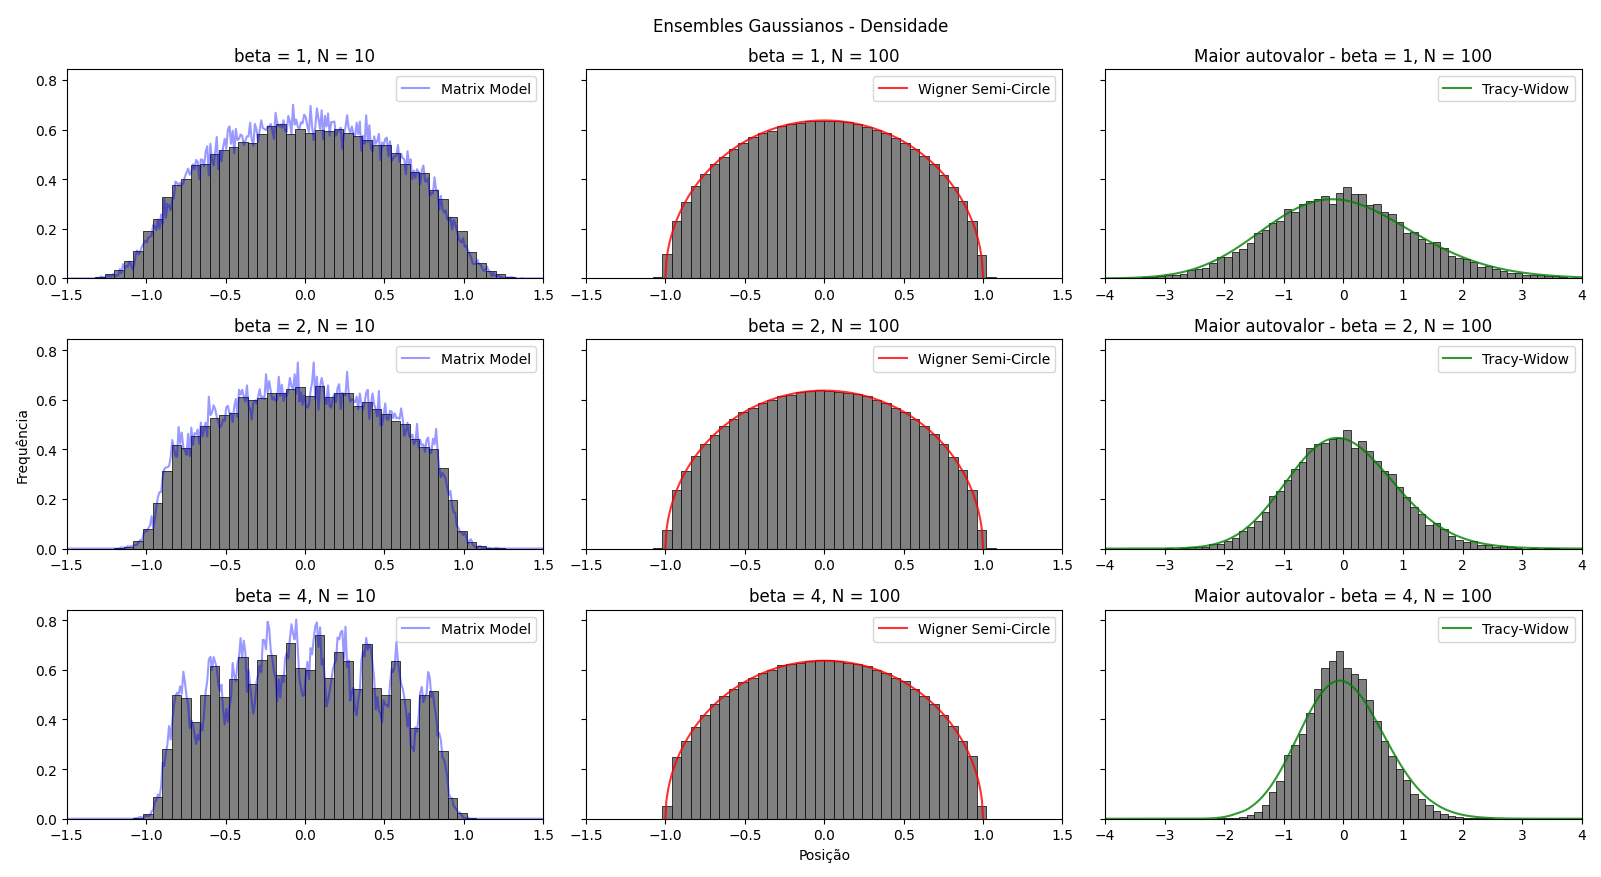
\includegraphics[width=\textwidth]{Assets/validationGaussianTracy.png}
	\caption{Densidade para ensembles gaussianos, \eqref{Equation: Parametros Gaussian}. Tomou-se $\Delta \tilde{t} = 0.1$ e $nsteps = 5\cdot10^6$ passos, registrando a cada $100$ iterações a partir de $nsteps/5$. À esquerda da figura, em azul, a densidade da amostragem de $4\cdot10^3$ matrizes do ensemble. No centro, o Semi-Círculo de Wigner, medida de equilíbrio. Na direita, apresenta-se a densidade de $\lambda_{max}$ normalizado e sua medida esperada.}
	\label{Figura: Gaussian}
\end{figure}

Podemos retomar também as descrições dos potenciais mônico e os dois regimes do potencial quártico. Respectivamente, estes modelos equivalem a tomar na simulação os parâmetros
\begin{equation}
	d = 1; \ \  n = 2; \ \ \V(x)= t |x|^{2m}; \ \ W(x) = g(x) = \log{|x|}; \ \ \beta_N = \beta N^2; \ \ \beta = 2.
	\label{Equation: Parametros Monico}
\end{equation}
\begin{equation}
	d = 1; \ \  n = 2; \ \ \V(x)=\frac{|x|^4}{4} + t \frac{|x|^2}{2}; \ \ W(x) = g(x) = \log{|x|}; \ \ \beta_N = \beta N^2; \ \ \beta = 2.
	\label{Equation: Parametros Quartico}
\end{equation}
O caso mônico se reduz ao gaussiano se $m=1$. Os resultados para ambos os potenciais estão explicitados na Figura \ref{Figura: Quartic Monic} para alguns parâmetros interessantes de $t$ e $m$.
\begin{figure}[ht!]
	\centering
	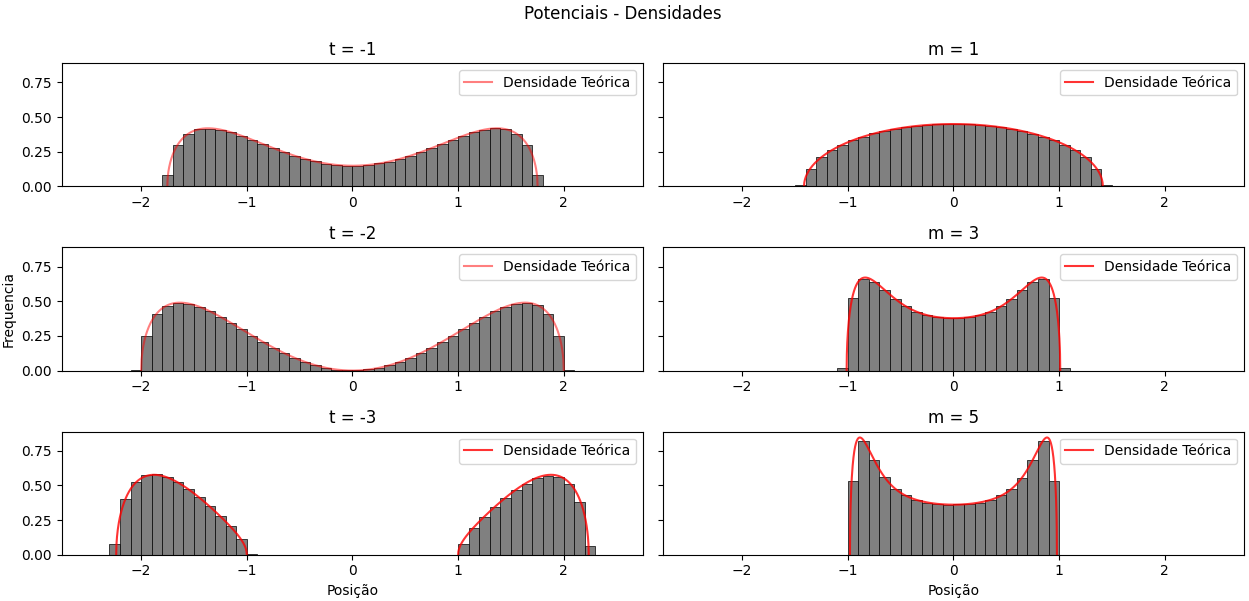
\includegraphics[width=\textwidth]{Assets/validationQuarticMonic-alt.png}
	\caption{Potencial Quártico \eqref{Equation: Parametros Quartico} e Mônico \eqref{Equation: Parametros Monico}, respectivamente à esquerda e direita. Tomou-se $\Delta \tilde{t} = 0.1$, $N=100$, e $nsteps = 5\cdot10^6$ passos. Registra-se a cada $1000$ iterações a partir de $nsteps/5$. No Quártico, simula-se $t=-1,-2,-3$. No Mônico fixa-se $t=1$ e simula-se $m=1,3,5$.}
	\label{Figura: Quartic Monic}
\end{figure}

Novamente as medidas experimentais parecem convergir para a medida teórica enunciada em todas as configurações testadas. Contudo, isso é discutido, com exceção do Mônico, por Chafa\"{i} e Ferré \cite{Chafa2018}. Em luz da situação recentemente explorada por Balogh \textit{et al.} \cite{balogh2016orthogonal} consideremos a Configuração \eqref{Equation: Complex} complexa. Para esta, representamos as medidas simuladas para alguns valores de interesse de $t, a$ na Figura \ref{Figura: Complex},
\begin{equation}
	d = 2; \  n = 2; \  \V(z)=|z|^{2a} - \Re{t z^a};  \ W(x) = g(x) = \log{|x|};  \ \beta_N = \beta N^2;  \ \beta = 2.
	\label{Equation: Complex}
\end{equation}

\begin{figure}[ht]
	\centering
	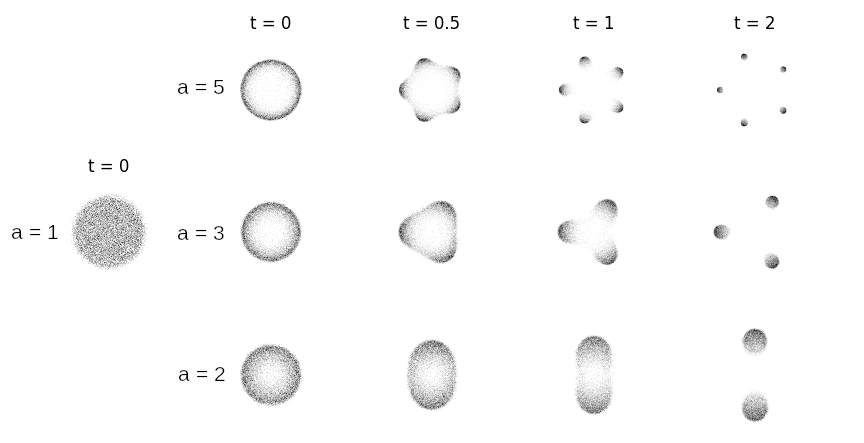
\includegraphics[width=0.75\textwidth]{Assets/complexPotential.png}
	\caption{Medidas referentes à configuração \eqref{Equation: Complex}. Tomou-se $\Delta \tilde{t} = 0.5$ e $nsteps = 2\cdot10^6$ passos, registrando a cada $500$ iterações a partir de $nsteps/5$.}
	\label{Figura: Complex}
\end{figure}

É previsto para esse modelo uma transição de regime - uma separação da medida de equilíbrio - para $t_c \approx \sqrt{a^{-1}}$, o que pode ser observado na Figura \ref{Figura: Complex} com algum detalhe. Outros fatores que corroboram o bom comportamento do modelo são que a medida é uniforme no disco quando $(a,t) = (1,0)$ e se concentra no bordo quando incrementa-se $a$, fatos também previstos. \cite{balogh2016orthogonal} Esse exemplo demonstra que é possível, sem muito esforço, replicar a medida, e principalmente o suporte, para potenciais mais complexos estudados em publicações recentes no tema e pode ser estendido para outros estudos, como para o potencial discutido por Bleher e Silva \cite{Silva}, dado pela Configuração \eqref{Equation: Silva}, representado em um diagrama de fase na Figura \ref{Figura: Silva}  
\begin{equation}
	d = 2; \  n = 2; \  \V(z)= t_0(|z|^{2} - 2\Re\{z^3/3 + t_1 z\});  \ W(x) = g(x) = \log{|x|}; \ \beta = 2.
	\label{Equation: Silva}
\end{equation}
\begin{figure}[ht]
	\centering
	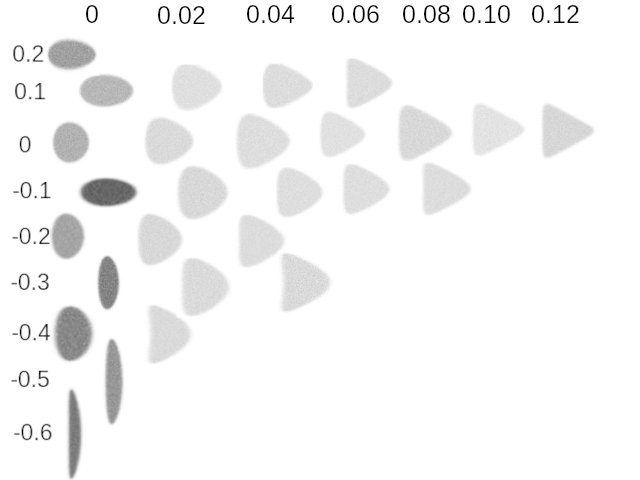
\includegraphics[width=0.7\textwidth]{Assets/allshapes.png}
	\caption{Medidas referentes à configuração \eqref{Equation: Complex}. Tomou-se $\Delta \tilde{t} = 0.5$ e $nsteps = 2\cdot10^6$ passos, registrando a cada $500$ iterações a partir de $nsteps/5$.}
	\label{Figura: Silva}
\end{figure}

\subsection{Conclusão}

A Teoria de Matrizes Aleatórias é uma ferramenta matemática extremamente versátil. Suas aplicações são extensas e diversas, cobrindo ambos sistemas físicos e matemáticos de grande relevância. Partindo da hipótese que autoenergias de sistemas complexos se comportam localmente como autovalores de matrizes aleatórias adequadas, permite-se a caracterização estatística do núcleo atômico ou ainda a determinação de propriedades físicas de metais. Em matemática, além das clássicas aplicações estatísticas dos modelos, mostra-se que matrizes aleatórias tem importante papel na determinação dos zeros da função de Riemann. Consolidada assim sua importância, a teoria se desenvolve rapidamente e tem chamado atenção da comunidade científica-matemática. Introduzimos neste trabalho as ideias de medida de matrizes aleatórias e ensembles, essenciais à RMT, e descrevemos os clássicos ensembles gaussianos, que julgamos exemplares para o entendimento dos resultados sobre medida nos autovalores e equilíbrio.

A analogia de Gases de Coulomb surge naturalmente ao se explicitar a medida de matrizes de ensembles invariantes. Sua interpretação permite pensar na dinâmica dos autovalores como uma de partículas interagentes, da qual intuímos as ideias de minimização da energia livre para identificar o equilíbrio. Percebemos que muitas vezes métodos numéricos são necessários para a solução das equações de movimento estocásticas que descrevem a dinâmica das partículas modeladas. Apresentamos então os métodos de simulação numérica e discutimos as principais características do algoritmo implementado, denominado \textit{Langevin Monte Carlo}.

Além disso, apresentamos os resultados, que dividimos, em propósito, em duas partes. Os primeiros resultados são de medidas de autovalores na reta, bem explorados na teoria e relativamente simples. Para estes, incluímos explicitamente no trabalho as soluções. Qualitativamente observa-se que os resultados tem boa concordância com a teoria, mesmo em distribuições mais delicadas, como a Tracy-Widow. Isso nos dá boa indicação do bom comportamento dos métodos e implementação utilizados. Com isso, apresentamos um dos resultados obtidos em um Gás de Coulomb em duas dimensões. Isso de refere a um potencial complexo, explorado com mais afinco apenas em teoria recente. Mesmo aqui, mostra-se que é possível replicar características de resultados apontados em trabalhos recentes e indica uma possível direção para exploração numérica da teoria.

Entendemos este estudo como uma descrição e validação de métodos conhecidos de simulação e matrizes aleatórias, ainda que atuais. Contudo, veem-se extensões da utilização do método para estudo numérico de importantes resultados com menos descrição teórica, o que, até onde sabemos, é menos explorado.

%%-----
%% Referências bibliográficas
%%-----
\addcontentsline{toc}{chapter}{\bibname}
\bibliographystyle{abntex2-num}
\bibliography{bibliografia}

%%-----
%% Fim do documento
%%-----

%\appendix
%\chapter{Implementação Algoritmo}

%\inputminted[
%frame=lines,
%framesep=2mm,
%baselinestretch=1.2,
%bgcolor=white,
%fontsize=\footnotesize,
%linenos
%]{FORTRAN}{Assets/HKMC.f}

\end{document}